\section{ОПТИМИЗАЦИЯ АЛГОРИТМА С ИСПОЛЬЗОВАНИЕМ CUDA}

Как и последовательная реализация решения задачи, оптимизированная с помощью CUDA реализация начинается с инициализации массивов, которая проводится таким же самым образом, как и в последовательной версии (см. Листинг \ref{listing:arrayInit}).

Далее необходимо отсортировать массивы по убыванию с помощью оптимизированной с помощью CUDA сортировки пузырьком. Идея оптимизации была позаимствована из статьи\footnote{\url{https://habr.com/en/post/235391/}} и заключается в том, что те элементы сортируемого массива, которые удалена от <<всплывающего>> элемента массива более, чем на 1 элемент, могут начать <<всплывать>>, при этом, его <<всплывание>> может происходит параллельно с <<всплыванием>> прочих элементов, достаточно от него удалённых. Каждое отдельное <<всплывание>> может производится на своем потоке. Реализация и её тонкости приведены в Листинге \ref{listing:bubbleSortCUDA}. Важно заметить, что у данной реализации сортировки пузырьком имеется параметр \texttt{blockSizeBubbleSort}, определяющий размер блоков при исполнении ядра.
\begin{lstlisting}[style=CStyle, label={listing:bubbleSortCUDA}, caption={Оптимизированная с помощью CUDA версия сортировки пузырьком.}]
/** Swaps elements idx and idx+1 if the element idx+1 is greater than the
 * 	element idx, if idx is lower than the current step by 2 and if idx is
 *  not n-1
 *  @param deviceArray Sorted array
 *	@param n Size of the sorted array
 * 	@param step Current step
 */ 
__global__ void bubbleSortKernel(float *deviceArray, int n, int step){
	// Thread linear id
	int idx = blockDim.x * blockIdx.x + threadIdx.x;
	float temp; // Temporary variable
	if (idx<(n-1)) {
    if ((step-2)>=idx){
      if (deviceArray[idx]<deviceArray[idx+1]){
        temp = deviceArray[idx];
        deviceArray[idx]=deviceArray[idx+1];
        deviceArray[idx+1] = temp;
      }
    }
  }
}

/** Sorts hostArray with the help of the Bubble sorting (CUDA is used)
 *	@param hostArray Sorted array
 *	@param n Size of the sorted array
 */
void bubbleSortCUDA(float *hostArray, int n){
	float *deviceArray; // declaration of a device copy of the sorted array
	cudaMalloc(&deviceArray, n * sizeof(float)); // Memory allocation
	// Copy host vector to device memory
	cudaMemcpy(deviceArray, hostArray, n*sizeof(float), cudaMemcpyHostToDevice);
	int gridSize = n / blockSizeBubbleSort + 1; // Size of a CUDA-grid
	// Bubble sort loop
	for (int step = 0; step <= n+n; step++){
		bubbleSortKernel<<<gridSize, blockSizeBubbleSort>>>(deviceArray, n, step);
		cudaThreadSynchronize();
	}
	// Copy back to host
	cudaMemcpy(hostArray, deviceArray, n*sizeof(float), cudaMemcpyDeviceToHost);
	// Release memory
	cudaFree(deviceArray);
}
\end{lstlisting}

Заключительной частью задачи является вычисление скалярного произведения отсортированных массивов. Идея оптимизации с помощью CUDA алгоритма вычисления скалярного произведения была взята с сайта\footnote{\url{http://cuda-programming.blogspot.com/2013/01/vector-dot-product-in-cuda-c.html}}. Вычисление может быть разбито на два этапа. На первом этапе вычисляются элементы массива $\vb{C}$ размера \texttt{gridDim}, содержащего промежуточный результат вычисления скалярного произведения. В каждом блоке декларируется в разделяемой памяти массив \texttt{cache[blockSize]}. Элемент массива с индексом \texttt{idx} (с индексом, равным линейному индексу данной нити) инициализируется нулём, затем к нему прибавляют произведения $\vb{A}[i]\cdot\vb{B}[i]$ для всех $i$ таких, что элементы массивов c индексом $i$, хранятся в памяти данной нити, то есть i = \texttt{idx}, \texttt{idx} + \texttt{blockDim.x * gridDim.x} и так далее. Когда в каждом из блоков посчитан массив \texttt{cache[blockSize]}, необходимо выполнить его суммирование. Для данной цели используется следующая схема, состоящая из нескольких шагов. Полагаем, что размер блока является степенью 2, тогда за первый шаг можно сложить в параллельном режиме две половинки массива (для определённости будем хранить результаты сложений в левой половинке), на следующем шаге мы уже складываем две половинки от первой половинки и так далее до тех пор, пока не дойдем до <<половинки>>, состоящей из единственного элемента. Один шаг такой схемы суммирования можно проиллюстрировать Рис. \ref{fig:sumReduction}.
\begin{figure}
    \centering
    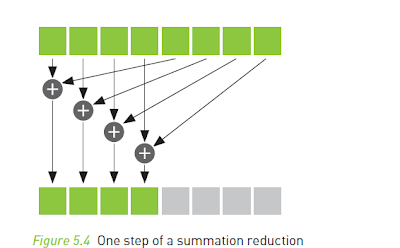
\includegraphics[scale=0.75]{fig/reduction+vector+dot+product.png}
    \caption{Один шаг сложения элементов массива \texttt{cache[blockSize]}.}
    \label{fig:sumReduction}
\end{figure}
Результат суммирования элементов массива \texttt{cache[blockSize]} для данного блока нитей будет лежать в элементе массива \texttt{cache[0]}. Если сложить элементы \texttt{cache[0]} всех блоков, то мы получим ответ! Однако, последний этап вычисления скалярного произведения оптимальнее производить на хосте, поэтому сохраним промежуточный результат в массив $\vb{C}$ следующим образом: \texttt{C[blockIdx.x] = cache[0]} (чтобы избежать конфликтов запись--запись, такую операцию необходимо выполнять на одной нити с одного блока).

Оптимизированный с помощью CUDA код может быть найден в Листинге \ref{listing:dotProdCUDA}, где функции с именами, имеющими на конце \texttt{CUDA} или \texttt{Kernel} относятся к оптимизированной версии алгоритма.
\begin{lstlisting}[style=CStyle, label={listing:dotProdCUDA}, caption={Оптимизированная с помощью CUDA версия вычисления скалярного произведения.}]
/** Computes intermediate result of dot product
 *	@param blockSize Size of a CUDA-block
 *	@param deviceA First vector
 *	@param deviceB Second vector
 *	@param deviceC Intermediate result
 *	@param n Size of the first and the second vectors
 */
template<int blockSize>
__global__ void dotProdKernel(float const *deviceA, float const *deviceB, float *deviceC, int n){
	// shared array for cache (this is a shared array for the whole threads in the current block)
	__shared__ float cache[blockSize];
	// Get our thread linear ID
  int idx = blockIdx.x * blockDim.x + threadIdx.x;
  float sum = 0;
  // Computation of sum of all elements that lie on this thread
  while (idx < n) {
  	sum += deviceA[idx] * deviceB[idx];
  	idx += blockDim.x * gridDim.x;
  }
  cache[threadIdx.x] = sum; // Filling cache
  __syncthreads(); // Barier synchronisation
  // Summation the cache (on the current block)
  int i = blockDim.x / 2;
  while (i != 0){
 		if (threadIdx.x < i) cache[threadIdx.x] += cache[threadIdx.x + i];
 		__syncthreads(); // Barier synchronisation
 		i /= 2;
 	}
 	// Sum of the cache on the current block is at cache[0] 
 	// Saving this result for each blocks
 	if (threadIdx.x == 0) deviceC[blockIdx.x] = cache[0];
}

/** Computes dot product (CUDA is used)
 *	@param hostA First array
 *	@param hostB Second array
 *	@param n Size of arrays
 */
float dotProdCUDA(float const *hostA, float const *hostB, int n){
	float *hostC; // declaration of vectors
	float *deviceA, *deviceB, *deviceC;
	// Number of thread blocks per grid
  int gridDimDotProd = (n + blockSizeDotProd - 1) / blockSizeDotProd;
  // Size in bytes of the vector C
  size_t bytesC = gridDimDotProd * sizeof(float);
	// Vectors allocation
	hostC = (float*)malloc(bytesC);
	cudaMalloc(&deviceA, n * sizeof(float));
  cudaMalloc(&deviceB, n * sizeof(float));
	cudaMalloc(&deviceC, bytesC);	
	// Copy host vectors to device
  cudaMemcpy(deviceA, hostA, n * sizeof(float), cudaMemcpyHostToDevice);
  cudaMemcpy(deviceB, hostB, n * sizeof(float), cudaMemcpyHostToDevice);
  // Execute the kernel
  dotProdKernel<blockSizeDotProd><<<gridDimDotProd, blockSizeDotProd>>>(deviceA, deviceB, deviceC, n);
  // Copy array back to host
  cudaMemcpy(hostC, deviceC, bytesC, cudaMemcpyDeviceToHost);
  // Release device memory
  cudaFree(deviceA);
  cudaFree(deviceB);
  cudaFree(deviceC);
  // Finish up on the host
  float res = 0;
  for (int i = 0; i < gridDimDotProd; i++){
  	res += hostC[i];
  }
  return res;
}
\end{lstlisting}
Следует заметить, что в оптимизированной с помощью CUDA версии вычисления скалярного произведения имеется один свободный параметр --- размер блока нитей \texttt{blockSizeDotProd}.